% multiple1902 <multiple1902@gmail.com>
% available on https://code.google.com/p/xjtu-cs-lect/
% licensed under cc by-sa 3.0
\setcounter{chapter}{-1}
\chapter{绪论}

\section{什么是组合数学}

    \textsf{组合数学}(combinatorial mathematics)是研究离散结构的存在, 计数, 分析和优化等问题的一门学科. 它

    \begin{itemize}
        \item (构造性)研究事物在给定模式下的配置(也称为方案),
        \item (存在性)研究这种配置(方案)是否存在
            \begin{itemize}
                \item 所有可能配置(方案)的数目和分类(计数),
                \item 配置(方案)的各种性质(优化).
            \end{itemize}
    \end{itemize}

\section{古代组合数学}

    组合数学源远流长, 但在远古时代这类问题往往联系着数的神秘主义出现. 

    \subsection{河图, 洛书}

        河图洛书, 来自上古时代有关数字排列之图案. 在宋朝之前, 洛书的记述只有文字, 一直到陈抟, 才提出了洛书的图案. 有人认为是重要的中国传统易理哲学部分, 后被广泛应用于风水、占卜等术数中. 
       
            \begin{figure}[!h]
                \centering
                \begin{minipage}[t]{.4\linewidth}
                    \centering
                    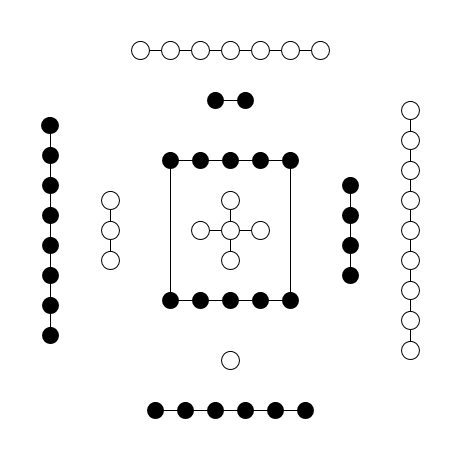
\includegraphics[width=.8\linewidth]{comb_notes/chap0_inc/河图.png}
                        % public domain
                    \caption{河图}
                    \label{fig:0:hetu}
                \end{minipage}
                \begin{minipage}[t]{.4\linewidth}
                    \centering
                    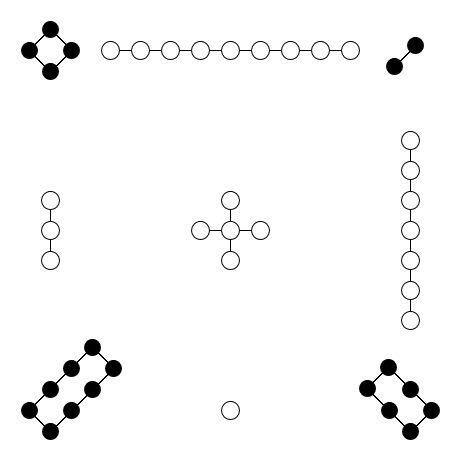
\includegraphics[width=.8\linewidth]{comb_notes/chap0_inc/洛书.png}
                        % public domain
                    \caption{洛书}
                    \label{fig:0:luoshu}
                \end{minipage}
            \end{figure}

